\documentclass[11pt,letterpaper]{article}
\usepackage[margin=0.72in]{geometry}
\usepackage{amsmath,amssymb,graphicx,booktabs,array}
\usepackage[T1]{fontenc}
\usepackage{lmodern}
\usepackage[hidelinks]{hyperref}
\setlength{\parindent}{0pt}
\setlength{\parskip}{4pt}
\setlength{\abovedisplayskip}{6pt}
\setlength{\belowdisplayskip}{6pt}
\setlength{\abovedisplayshortskip}{4pt}
\setlength{\belowdisplayshortskip}{4pt}
\newcommand{\sech}{\operatorname{sech}}
\newcommand{\WireA}{0.198992}
\newcommand{\WireB}{0.199601}
\newcommand{\WireD}{1.003060}
\newcommand{\WireKernel}{20.439}
\newcommand{\WireEquation}{0.383}
\newcommand{\WireDirect}{0.056}
\newcommand{\NoiselessEquation}{0.353}
\newcommand{\SparseEquation}{6.23}
\newcommand{\WedgeInside}{0.158}
\newcommand{\WedgeOutside}{0.961}
\newcommand{\TanhAmplitude}{1.699495}
\newcommand{\TanhLength}{0.899139}
\newcommand{\TanhCenter}{-0.000644}
\newcommand{\TanhError}{0.045}
\newcommand{\SensorKernel}{8.090}
\newcommand{\SensorEquation}{5.225}
\newcommand{\SensorDirect}{5.312}

\hypersetup{pdftitle={Maxwell's Perspective: Observations, learned kernels and the analytic functions we infer},
pdfauthor={J. R. Landers},
pdfsubject={An expository companion connecting kernel-to-equation discovery, measured magnetic reconstruction, and a hidden-wire experiment}}
\begin{document}
\begin{center}
{\Large\bfseries Maxwell's Perspective}\\[3pt]
{\large Observations, learned kernels and the analytic functions we infer}\\[3pt]
{\small J. R. Landers\quad$\cdot$\quad November 2026}
\end{center}
\vspace{-6pt}

\textbf{Starting question.}
If two observers meet the same magnetic world through different experiments and
different mathematical tools, will they arrive at the same analytic function?
Our first two notes~[1,2] approached this question operationally: learn a predictor
from observations, translate it into mathematics, construct an explicit function,
and test what that function predicts. A new hidden-wire experiment lets us place
the recovered expression beside a known theoretical solution. Their close
agreement is a useful result. The way that agreement was obtained is the subject
of this note.

\textbf{1. A perspective before a formula.}
Imagine receiving a table of positions, currents and compass-like readings.
The field's formula is absent. You can interpolate the table, draw curves through
it, propose relationships, and ask what another observation would show.
Every step introduces a representation. Eventually a short equation may do what
the table could not: describe a whole family of observations at once.

This is the sense in which we borrow ``Maxwell's perspective.'' In his work on
physical lines of force, Maxwell compared mechanical hypotheses with observed
magnetic and electrical phenomena~[3]. His later field theory joined experimentally
motivated relations and connected electromagnetic disturbances with light~[4].
Our experiment reproduces one inference problem, not that historical achievement.
Maxwell's intermediates included field pictures, analogies and mathematical
constraints; ours include a kernel predictor and a finite expression search.
Both routes connect observations to mathematical consequences.

In modern vacuum notation, one relevant field equation is
\begin{equation}
\nabla\times\mathbf B
=\mu_0\mathbf J+\mu_0\epsilon_0\frac{\partial\mathbf E}{\partial t}.
\label{eq:ampere}
\end{equation}
Here $\mathbf E$ and $\mathbf B$ are electric and magnetic fields, $\mathbf J$ is
current density, and $\mu_0,\epsilon_0$ are vacuum constants. Under steady conditions,
an ideal infinite straight wire and cylindrical symmetry give
\begin{equation}
\oint\mathbf B\cdot d\boldsymbol\ell=\mu_0 I,
\qquad B_\varphi(r)=\frac{\mu_0 I}{2\pi r}.
\label{eq:wire}
\end{equation}
$I$ is the enclosed signed current, $r$ distance from the wire, and $\varphi$
the direction around it. This familiar solution follows from the steady
Amp\`ere law together with geometry. It is not the full Maxwell system.

\textbf{2. Put the functions beside each other.}
For positions $x,y$ in metres, current $I$ in amperes and fields in microtesla,
our simulator uses the coefficient 0.2. The first fixed 1\%-noise run recovers:
\begin{equation}
\begin{array}{c@{\qquad\qquad}c}
\text{Hidden ideal-wire field}&\text{Kernel-derived analytic field}\\[5pt]
\displaystyle\mathbf B_*=
\frac{0.2I}{x^2+y^2}\begin{pmatrix}-y\\x\\0\end{pmatrix}
&\displaystyle\mathbf B_\theta=
\frac{I}{\WireD x^2+y^2}
\begin{pmatrix}-\WireA y\\\WireB x\\0\end{pmatrix}.
\end{array}
\label{eq:pair}
\end{equation}
The same algebraic structure has emerged, with small coefficient differences.
The learner was given neither expression. The displayed decimals are rounded;
all scores use the saved full-precision function. Agreement here concerns one
particular magnetic response, within a supplied algebraic search class.
The simulated world obeys the wire law by construction; recovering it tests
our inference process without independently validating electromagnetism.

\newpage
\textbf{3. Three experiments, one operational arc.}
The shared route is
\begin{equation}
\text{data}\ \longrightarrow\ \text{kernel}
\ \longrightarrow\ \text{mathematical structure}
\ \longrightarrow\ \text{analytic function}\ \longrightarrow\ \text{test}.
\label{eq:workflow}
\end{equation}
For an input $\mathbf u$, the common predictor has the form
\begin{equation}
\widehat{\mathbf B}_K(\mathbf u)
=\overline{\mathbf B}+\sum_n k_\ell(\mathbf u,\mathbf u_n)\boldsymbol\alpha_n,
\qquad
k_\ell=\exp\!\left[-\frac{\|S^{-1}(\mathbf u-\mathbf u_n)\|^2}{2\ell^2}\right].
\label{eq:kernel}
\end{equation}
The coefficients come from regularized fitting. Validation selects the smoothing
length $\ell$ and penalty. In the wire study $S$ contains training input standard
deviations; the earlier spatial studies use their stated coordinate scales.
The similarity kernel supplies smoothness, not a magnetic field law.

\begin{center}
\small
\begin{tabular}{@{}>{\raggedright\arraybackslash}p{.16\linewidth}>{\raggedright\arraybackslash}p{.25\linewidth}>{\raggedright\arraybackslash}p{.25\linewidth}>{\raggedright\arraybackslash}p{.26\linewidth}@{}}
\toprule
& Note 1: hidden profile & Note 2: measured room & This note: hidden wire\\
\midrule
Observations & Dimensionless $B(x),J(x)$ samples & Planar positions and three magnetic channels & Cartesian positions, signed current and three magnetic channels\\[3pt]
Bridge & Sparse differential equation & Supplied magnetic dipole response & Sparse polynomial/rational search\\[3pt]
Construct & Solve the selected ODE & Assemble equivalent sources & Evaluate the selected rational function\\[3pt]
Judge & Hidden analytic profile & Held-out measured readings & Hidden field at unseen conditions\\
\bottomrule
\end{tabular}
\end{center}
\vspace{-4pt}

In note~1, a field-only search selects $B'=p-qB^2$. Separation of variables,
on the branch fixed by a learned reference value, yields
\begin{equation}
B_{\rm sym}(x)=A\tanh\!\left(\frac{x-x_c}{L}\right),\qquad
A=\sqrt{p/q},\quad L=(pq)^{-1/2}.
\label{eq:tanh}
\end{equation}
The hidden profile has $(A,L,x_c)=(1.7,0.9,0)$. The noisy recovery gives
$(\TanhAmplitude,\TanhLength,\TanhCenter)$, with \TanhError\% field error.
The equation grammar and integration rule are supplied; the selected equation,
scales and center are inferred. The companion source recovers a $\sech^2$ shape.

In note~2, public Aalto recordings~[5] supply real vector measurements, but no
analytic room-field oracle. A theoretical representation replaces the ODE:
\begin{equation}
\mathbf B_D(\mathbf r)=\mathbf b_0+
\sum_j\left(\frac{3\mathbf R_j\mathbf R_j^{\mathsf T}}{R_j^5}
-\frac{\mathbb I_3}{R_j^3}\right)\mathbf q_j,
\qquad\mathbf R_j=\mathbf r-\mathbf s_j.
\label{eq:dipole}
\end{equation}
The source positions $\mathbf s_j$ belong to an assumed subsurface grid;
effective moments $\mathbf q_j$ and background $\mathbf b_0$ are fitted to kernel
outputs. The source-free magnetic structure is supplied. Stable reference-sensor
RMSE falls from \SensorKernel\ to \SensorEquation; a direct-data dipole control
gives \SensorDirect, in recording units. Equivalent sources do not identify the
room's actual objects, and planar observations do not fix a unique 3D field.

For the wire, we supply general monomials
$\boldsymbol\phi_d=\{x^a y^b I^c:a+b+c\leq d\}$ instead of dipoles. The candidate is
\begin{equation}
B_{\theta,j}(\mathbf u)=
\frac{\boldsymbol\phi_d(\mathbf u)^{\mathsf T}\mathbf p_j}
{\boldsymbol\phi_d(\mathbf u)^{\mathsf T}\mathbf q},\qquad
t_{n,j}Q(\mathbf u_n)-P_j(\mathbf u_n)\approx0,
\quad \mathbf t_n=\widehat{\mathbf B}_K(\mathbf u_n).
\label{eq:rational}
\end{equation}
Sparse homogeneous fitting and field-value refinement construct the candidate;
validation observations select it. Polynomials are also allowed. As in note~2,
targets are teacher values at actual training inputs, not extra observations.
The extracted expression is a new model, not an exact symbolic rewrite of
the Gaussian sum.

\newpage
\textbf{4. What happened when the world was hidden?}
We fit 480 training observations, validate on 180, and score 800 independent
points per test. The main domain has radii 0.25--2~m, all angles and
$|I|=0.5$--4~A. Main noise is independent Gaussian noise per component, with
standard deviation 1\% of pooled clean training component RMS; its scale is
withheld from selection. Three fixed seeds are run for each of five conditions:
no noise, 1\% noise, 5\% noise, 80 training points, and a restricted angular wedge.

The learner sees $x,y,I$ and $B_x,B_y,B_z$, with no radial features, derivatives
or permeability. Validation selects among Gaussian kernels, then among general
polynomials through degree~4 and rational expressions through degree~2.
The sparsest expression within 5\% of the best validation MSE is retained,
with a fixed numerical floor. The identical expression search is independently
repeated on raw observations. All choices finish before test labels are opened.

\begin{center}
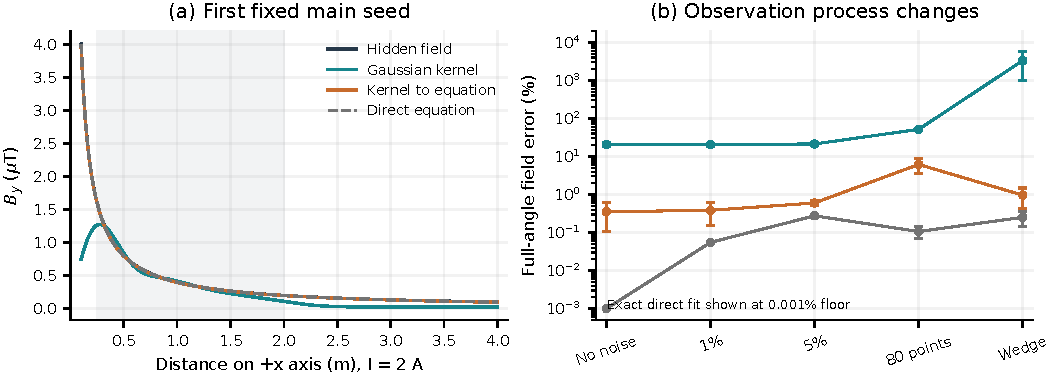
\includegraphics[width=\linewidth]{perspective.pdf}
\end{center}
\vspace{-9pt}
{\small\textbf{Figure 1.} (a) A fixed cut at $y=0$, $I=2$~A, for the first main
seed; shading marks the observed radius range. (b) Full-angle errors under five
observation conditions; points and bars are means and standard deviations across
three seeds. ``Wedge'' training/validation sees only angles $\pm\pi/6$.
The noiseless direct fit is at numerical precision and displayed at the stated
floor. All selected expressions, including failures of accurate coefficient
recovery, are retained in the experiment archive.}

\vspace{4pt}
The main-case table reports $100\|\mathbf B_{\rm model}-\mathbf B_*\|_2/
\|\mathbf B_*\|_2$, averaged over all three seeds:
\begin{center}
\small\begin{tabular}{@{}lrrr@{}}
\toprule
Unseen conditions & Kernel & Kernel $\to$ equation & Direct equation \\
\midrule
Same domain & 20.439 & 0.383 & 0.056 \\
Smaller radii & 71.538 & 0.381 & 0.056 \\
Larger radii & 97.839 & 0.379 & 0.055 \\
Larger currents & 97.366 & 0.380 & 0.055 \\
Moved wire; no update & 86.991 & 89.869 & 89.999 \\
\bottomrule
\end{tabular}

\end{center}
\vspace{-4pt}
The extracted fields recover the wire's monomial support in all 15 runs.
Current proportionality and inverse-distance scaling follow exactly from that
selected support; circular symmetry is approximate because coefficients differ.
Errors remain small beyond the observed distances and currents. Yet direct
equation fitting is better: \WireDirect\% versus \WireEquation\% in the main
domain. The kernel stage is not shown necessary. Its main fits select the smallest
searched length, so its \WireKernel\% error is a result for this search, not an
established optimum for kernel learning.
Even without measurement noise, the finite kernel-to-equation route retains
\NoiselessEquation\% mean field error; exact samples do not remove its approximation choices.

Sparse sampling increases the distilled error to \SparseEquation\%.
Wedge-only observations give \WedgeInside\% within the wedge and
\WedgeOutside\% over all angles. A nonmagnetic polynomial control recovers a
polynomial, rather than a wire shape. Moving the wire without supplying its new
position defeats all frozen models. These outcomes measure what the process
retains, what its grammar can express, and which changing conditions its inputs omit.

\newpage
\textbf{5. The experiment helps define the function.}
A measurement is already a relationship between a world and an apparatus.
Write an experiment's observations schematically as
\begin{equation}
\mathbf b_i=H_e[F](\mathbf u_i)+\boldsymbol\epsilon_i,
\qquad
f_e^*(\mathbf u)=\mathbb E[\mathbf b\mid\mathbf u,e].
\label{eq:observation}
\end{equation}
$F$ denotes a candidate physical state or field history; $H_e$ includes the
channels, calibration, orientation and averaging of experiment $e$.
For squared prediction loss, the population target is the conditional mean
$f_e^*$. A finite learner approximates it through its chosen representation.
Changing the available inputs or the observation operator can change that target,
even when the physical world is unchanged.

The wire gives a sharp example. Keep both signs of current but remove $I$ from
the learner's inputs. If its conditional mean is zero, then
\begin{equation}
\mathbb E[\mathbf B_*\mid x,y]
=\frac{0.2\,\mathbb E[I\mid x,y]}{x^2+y^2}(-y,x,0)=\mathbf0.
\label{eq:missing}
\end{equation}
Zero is then the optimal mean predictor for those incomplete inputs. Individual
readings still have nonzero fields and irreducible error for that predictor.
The zero function and the current-conditioned wire function answer different
statistical questions. This is a theoretical consequence of the setup, not an
additional fitted experiment. Similarly, spatial averages, missing orientation
or magnetic history can require a different effective description.

\textbf{6. Would the two routes converge?}
They can converge in predictive content if they target the same calibrated
quantity, include the relevant conditions, sample a sufficiently informative
domain, and use representations and estimators capable of consistent recovery.
They need not converge to identical notation. For two experimental routes,
observational equivalence over a tested domain means
\begin{equation}
F_1\sim F_2\quad\Longleftrightarrow\quad
H_e[F_1](\mathbf u)=H_e[F_2](\mathbf u)
\quad\text{for every tested }(e,\mathbf u).
\label{eq:equivalence}
\end{equation}
This identifies a unique field only when those observations distinguish the
candidate fields. Finite noisy samples generally leave alternatives; the planar
sensor study particularly leaves unobserved 3D structure. Differential equations,
source expansions and integral kernels may also express the same field while
retaining different parameters. Our small wire experiment demonstrates close
recovery within its grammar, not a convergence theorem.

Neither an analytic expression nor an ML predictor becomes ``more real'' through
its form. Both earn empirical scope by surviving tests. Maxwell's equations carry
claims across many configurations; one recovered wire function addresses a narrow
slice. Two functions may be equally adequate on that slice and disagree elsewhere.
Their disagreement gives the next experiment: vary the source geometry, resolve
a missing direction, or observe time dependence and induction. A useful theory
connects those experiments with fewer new assumptions.

\textbf{Takeaway.}
The three studies make an empirical route to explicit mathematics inspectable.
The function we recover depends jointly on observations, accessible variables and
mathematical choices. Our wire expressions nearly meet at a familiar law; our
sensor reconstruction supplies a physical family; our first note solves a selected
equation. The next question is which recovered relationships remain stable when
the experiment changes. That stability can support a shared theory without
requiring a privileged formula or a unique hidden source arrangement.

\vfill
{\footnotesize\raggedright
\textbf{References and reproducibility.}\par
[1] J.~R. Landers, \href{../01-kernel-to-equation/kernel_to_equation.pdf}{\emph{From samples to an equation}}
(2026).\quad
[2] J.~R. Landers, \href{../02-kernel-to-magnetostatics/kernel_to_magnetostatics.pdf}{\emph{From a learned kernel to a magnetic field}}
(2026).\par
[3] J.~C. Maxwell, \href{https://en.wikisource.org/wiki/On_Physical_Lines_of_Force}{\emph{On physical lines of force}}
(1861--62), opening discussion.\par
[4] J.~C. Maxwell, \emph{A dynamical theory of the electromagnetic field} (1865),
\href{https://doi.org/10.1098/rstl.1865.0008}{doi:10.1098/rstl.1865.0008};
\href{https://en.wikisource.org/wiki/A_Dynamical_Theory_of_the_Electromagnetic_Field/Part_I}{Parts I}
and \href{https://en.wikisource.org/wiki/A_Dynamical_Theory_of_the_Electromagnetic_Field/Part_VI}{VI}.\par
[5] A. Solin et al., \emph{Modeling and interpolation of the ambient magnetic field
by Gaussian processes} (2018),
\href{https://doi.org/10.1109/TRO.2018.2830326}{doi:10.1109/TRO.2018.2830326}.\par
Protocol, all fits, sensor-stage audit and tests: \texttt{experiments/hidden\_wire/}.
Build all notes: \texttt{python scripts/build\_papers.py}.\par}
\end{document}
